\documentclass[tikz, border=2mm]{standalone}
\usepackage{bm}

\begin{document}
    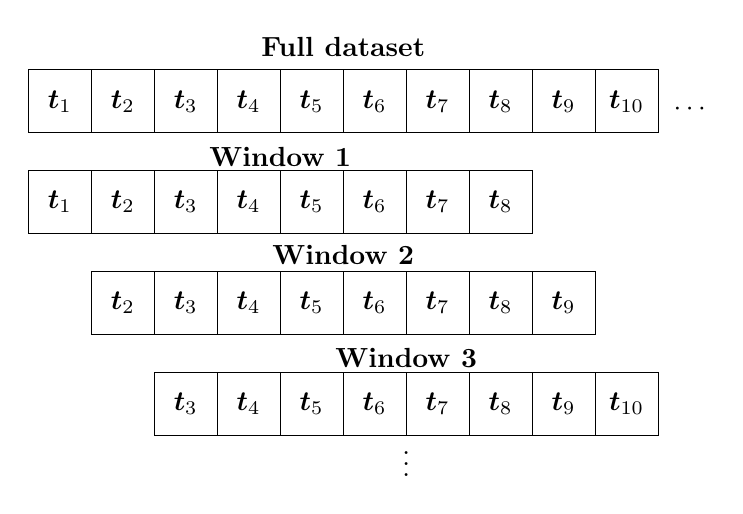
\begin{tikzpicture}
        \def\boxsize{0.8cm}
        \tikzstyle{box} = [draw, minimum size=\boxsize, node distance=0.05cm]
        \tikzstyle{label} = [above, font=\bfseries]
        % Draw a label "full dataset"
        \node[label] at (5.5*\boxsize, 0.45) {Full dataset};
        % Draw 10 boxes in a row for the full dataset
        \foreach \j in {1,...,10} {
            \node[box] (box\j) at (\j*\boxsize, 0) {$\bm{t}_{\j}$};
        }
        % Draw some cdots to show that the dataset continues past t_10
        \node (boxdots) at (11*\boxsize, -0.1) {$\cdots$};
        % Draw a label for "window 1"
        \node[label] at (4.5*\boxsize, -0.95) {Window 1};
        % Draw the boxes for the first window
        \foreach \j in {1,...,8} {
            \node[box] (box2\j) at (\j*\boxsize, -1.6*\boxsize) {$\bm{t}_{\j}$};
        }
        % Draw a label for "window 2"
        \node[label] at (5.5*\boxsize, -2.2) {Window 2};
        % Draw the boxes for the second window
        \foreach \j in {2,...,9} {
            \node[box] (box3\j) at (\j*\boxsize, -3.2*\boxsize) {$\bm{t}_{\j}$};
        }
        % Draw a label for "window 3"
        \node[label] at (6.5*\boxsize, -3.5) {Window 3};
        % Draw the boxes for the third window
        \foreach \j in {3,...,10} {
            \node[box] (box4\j) at (\j*\boxsize, -4.8*\boxsize) {$\bm{t}_{\j}$};
        }
        % Draw some vdots to indicate that the windows continue
        \node (boxvdots) at (6.5*\boxsize, -4.5) {$\vdots$};

    \end{tikzpicture}
\end{document}
